\section{Datasets and Experimental results analysis} \label{section4}
The experiments use the traffic accident detection dataset hosted on Hugging Face \cite{hiennguyen2024accident}. The public dataset provides images, object annotations, image dimensions, and image-level accident flags; it does not directly provide CRT targets, TTC values, or intervention levels. These labels were derived by our preprocessing pipeline. For the experiments reported here, we used 3,000 scenes for training and 600 for validation, then used 120 validation scenes for the ablation study and PIKV analysis. These are the splits used in our experiments, rather than separate official train and validation splits supplied by the dataset. Table~\ref{table_datasets} summarises them.

% TODO before submission: document the exact CRT-target construction, the mapping from targets to levels (0--4), the scene-selection procedure and random seed, and what the table's "40 quick" subset means. Verify the bibliography entry and dataset license against the dataset card; these details were not present in the supplied experiment description.

\begin{table}[H]
\caption{Data used in our experiments.}
\centering
\label{table_datasets}
\adjustbox{max width=\linewidth}{
\begin{tabular}{l|c|c|l|l}
\hline
\textbf{Data} & \textbf{Split} & \textbf{Samples} & \textbf{Used For} & \textbf{Labels} \\
\hline
Traffic accident detection \cite{hiennguyen2024accident} & Train (our split) & 3,000 scenes & Training (5 epochs) & Derived CRT target, level (0--4) \\
Traffic accident detection \cite{hiennguyen2024accident} & Validation (our split) & 600 scenes & Model selection & Derived CRT target, level (0--4) \\
Traffic accident detection \cite{hiennguyen2024accident} & Validation subset & 120 (40 quick) & Ablation, PIKV pruning & Derived anomaly label if CRT$^{*} > 0.4$ \\
Scripted demo scenarios A--D & -- & 4 scenarios & Behaviour check & Expected level \\
\hline
\end{tabular}
}
\end{table}

\textbf{Setup.} We used PyTorch 2.6.0 and CUDA 12.4 on an Intel i7-12700H system with 16~GB RAM and an NVIDIA RTX 3050 Laptop GPU (4~GB VRAM). AdamW was used with learning rate $3 \times 10^{-4}$ and batch size 16. A sample was labelled as an anomaly when CRT $> 0.4$. The TTC-only baseline used the threshold $\min_i \text{TTC}_i < 3$~s. The configured vehicle limits were $\mu g=6.867$~m/s$^2$, $a_{\text{lat,max}}=6.0$~m/s$^2$, and $\dot{\psi}_{\max}=1.2$~rad/s. These thresholds, together with the 30~FPS reference and 10~ms per-frame target used below, are design settings for this experiment; they were not learned from the cited dataset.

\textbf{Training behaviour.} Figure~\ref{fig_training} shows the loss and CRT MAE across five epochs. Validation loss reached 0.0396 and CRT MAE reached 0.0417. The training log reports 100\% validation accuracy from epoch 1, but the available notes do not identify whether this score uses all 600 validation scenes or the 120-scene ablation subset. We therefore do not treat this figure alone as evidence of generalisation. The class imbalance measured in the 120-scene subset is discussed below.

% TODO before submission: identify the exact evaluation subset used for the epoch-1 accuracy, and check whether CRT targets are derived from any feature also supplied to the model (possible label leakage).

\begin{figure}[H]
\centering
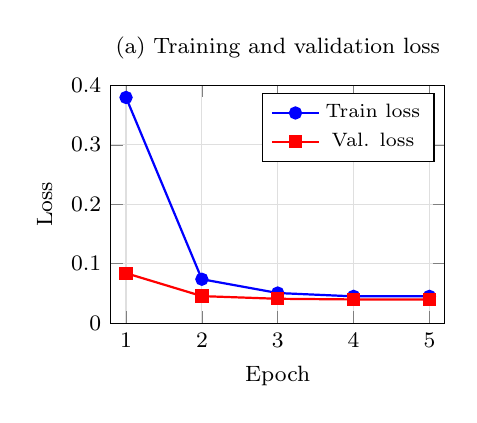
\begin{tikzpicture}
\begin{axis}[
    width=0.48\linewidth, height=4.6cm,
    xlabel={Epoch}, ylabel={Loss},
    xmin=0.8, xmax=5.2, ymin=0, ymax=0.4, xtick={1,2,3,4,5},
    grid=major, grid style={gray!25},
    legend style={font=\scriptsize}, legend pos=north east,
    tick label style={font=\footnotesize}, label style={font=\footnotesize},
    title={\footnotesize (a) Training and validation loss}]
\addplot[thick, blue, mark=*] coordinates {(1,0.3797) (2,0.0738) (3,0.0506) (4,0.0450) (5,0.0450)};
\addlegendentry{Train loss}
\addplot[thick, red, mark=square*] coordinates {(1,0.0840) (2,0.0454) (3,0.0409) (4,0.0398) (5,0.0396)};
\addlegendentry{Val. loss}
\end{axis}
\end{tikzpicture}
\hfill
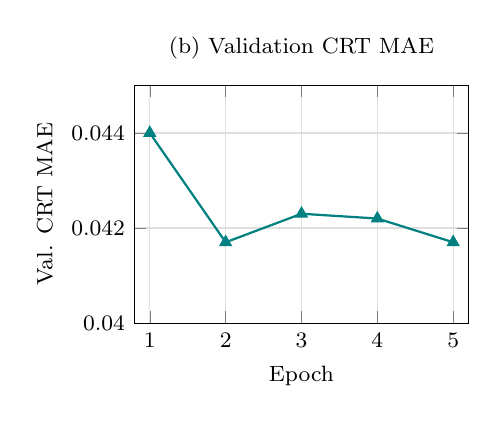
\begin{tikzpicture}
\begin{axis}[
    width=0.48\linewidth, height=4.6cm,
    xlabel={Epoch}, ylabel={Val. CRT MAE},
    xmin=0.8, xmax=5.2, ymin=0.040, ymax=0.045, xtick={1,2,3,4,5},
    yticklabel style={/pgf/number format/fixed, /pgf/number format/precision=3},
    scaled y ticks=false,
    grid=major, grid style={gray!25},
    tick label style={font=\footnotesize}, label style={font=\footnotesize},
    title={\footnotesize (b) Validation CRT MAE}]
\addplot[thick, teal, mark=triangle*] coordinates {(1,0.0440) (2,0.0417) (3,0.0423) (4,0.0422) (5,0.0417)};
\end{axis}
\end{tikzpicture}
\captionsetup{singlelinecheck = false, format= hang, justification=justified, font=footnotesize, labelsep=space}
\caption{Training history of PC-CSG on the traffic accident detection dataset \cite{hiennguyen2024accident} (3,000 training / 600 validation scenes, AdamW, learning rate $3 \times 10^{-4}$, batch size 16).}
\label{fig_training}
\end{figure}

\subsection{Hardware Profiling and Latency Breakdown}
We profiled the pipeline on an RTX 3050 Laptop GPU using 10 agents, 6 counterfactuals, and 15 horizon steps. Table~\ref{table_latency} and Figure~\ref{fig_latency} report the measured times. In this configuration, the pipeline reached 149.7~FPS. With hidden dimension $D=128$, the CSGA forward pass took 1.57~ms. No measurement was made on an embedded automotive platform, so the laptop result should not be read as an embedded-device benchmark.

\begin{table}[H]
\caption{Measured component-level inference latency on an NVIDIA RTX 3050 Laptop GPU ($N=10$ agents, $K=6$ counterfactuals, $H=15$ horizon).}
\centering
\label{table_latency}
\begin{tabular}{l|c|c}
\hline
\textbf{Pipeline Component} & \textbf{Latency (ms)} & \textbf{Share (\%)} \\
\hline
Scene Graph Construction \& Hazard Scoring & 0.33~ms & 4.9\% \\
Counterfactual Scene Graph Attention (CSGA) & 1.57~ms & 23.5\% \\
Kinematic Bicycle Model Propagation ($N \times K$) & 4.12~ms & 61.7\% \\
Physics-Informed Kinematic Validator (PIKV) & 0.53~ms & 7.9\% \\
CRT Engine \& Intervention Arbiter & 0.13~ms & 1.9\% \\
\hline
\textbf{Total PC-CSG Pipeline Latency} & \textbf{6.68~ms} & \textbf{100.0\%} \\
\textbf{Effective Real-Time Throughput} & \multicolumn{2}{c}{\textbf{149.7 FPS}} \\
\textbf{Throughput vs. 30 FPS reference target} & \multicolumn{2}{c}{\textbf{4.99$\times$ Real-Time Throughput}} \\
\hline
\end{tabular}
\end{table}

\begin{figure}[H]
\centering
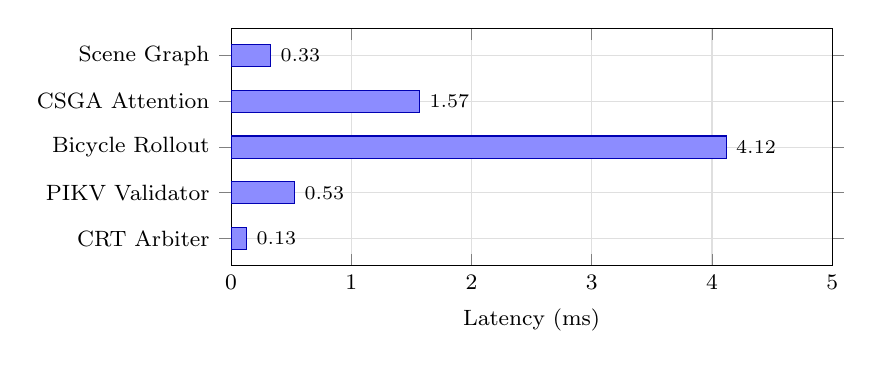
\begin{tikzpicture}
\begin{axis}[
    xbar, width=0.76\linewidth, height=4.6cm,
    xlabel={Latency (ms)}, xmin=0, xmax=5,
    ytick={1,2,3,4,5},
    yticklabels={CRT Arbiter, PIKV Validator, Bicycle Rollout, CSGA Attention, Scene Graph},
    y dir=normal, bar width=8pt, enlarge y limits=0.15,
    nodes near coords, nodes near coords align={horizontal},
    every node near coord/.append style={font=\scriptsize},
    tick label style={font=\footnotesize}, label style={font=\footnotesize},
    grid=major, grid style={gray!25}]
\addplot[fill=blue!45, draw=blue!70!black] coordinates {(0.13,1) (0.53,2) (4.12,3) (1.57,4) (0.33,5)};
\end{axis}
\end{tikzpicture}
\captionsetup{singlelinecheck = false, format= hang, justification=justified, font=footnotesize, labelsep=space}
\caption{Component-level latency of PC-CSG on an NVIDIA RTX 3050 Laptop GPU (total 6.68~ms, 149.7~FPS).}
\label{fig_latency}
\end{figure}

The measured end-to-end latency was 6.68~ms, equivalent to 149.7~FPS. This is above the 30~FPS reference target and below the separate 10~ms per-frame design target. The bicycle rollout took 4.12~ms (61.7\% of the total), while CSGA took 1.57~ms. A Python loop launches small GPU kernels over the 15 rollout steps and contributes to the cost; combining these operations with \texttt{torch.compile} may reduce the overhead, but that improvement has not yet been measured.

\subsection{PIKV Validation Effectiveness}
The 120 validation scenes contained 113 critical vehicles, from which the system generated 678 counterfactual hypotheses. PIKV filtered out 312 hypotheses (\textbf{46.0\%}) in total. The results for each mode appear in Table~\ref{table_pruning} and Figure~\ref{fig_pikv}.

\begin{table}[H]
\caption{PIKV hypothesis pruning across the six counterfactual modes (678 hypotheses, 113 per mode, from real traffic validation samples).}
\label{table_pruning}
\centering
\adjustbox{max width=\linewidth}{
\begin{tabular}{l|c|l}
\hline
\textbf{Counterfactual Mode} & \textbf{Pruning Rate} & \textbf{Main Rejection Reason} \\
\hline
\texttt{sudden\_brake} & 0.0\% & Straight-line deceleration stays inside the friction circle \\
\texttt{hard\_swerve\_left} & 70.8\% & Lateral acceleration exceeds $a_{\text{lat,max}}$ / friction circle \\
\texttt{hard\_swerve\_right} & 21.2\% & Rejected only when path curvature breaks friction limits \\
\texttt{sudden\_acceleration} & 100.0\% & Surge combined with learned steering breaks $a_{\text{total}} \le \mu g$ \\
\texttt{lane\_departure} & 73.5\% & Yaw rate exceeds $\dot{\psi}_{\max} = 1.2$~rad/s \\
\texttt{stationary\_obstacle} & 10.6\% & Feasible unless stopping needs more than the available deceleration \\
\hline
\textbf{Overall Pruning Rate} & \textbf{46.0\%} & \textbf{312 / 678 hypotheses filtered} \\
\hline
\end{tabular}
}
\end{table}

\begin{figure}[H]
\centering
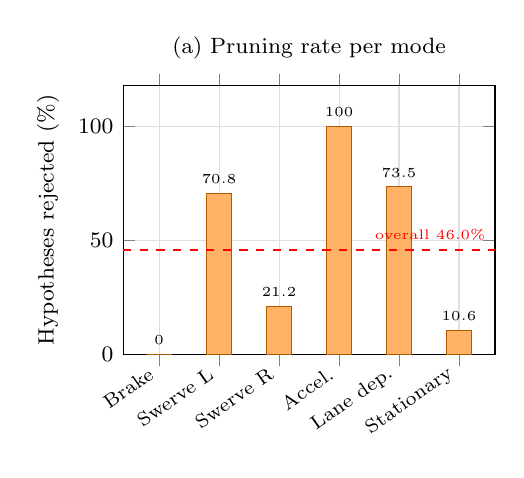
\begin{tikzpicture}
\begin{axis}[
    ybar, width=0.52\linewidth, height=5.0cm,
    ylabel={Hypotheses rejected (\%)}, ymin=0, ymax=118,
    xtick={1,2,3,4,5,6},
    xticklabels={Brake, Swerve L, Swerve R, Accel., Lane dep., Stationary},
    x tick label style={rotate=35, anchor=east, font=\scriptsize},
    xmin=0.4, xmax=6.6, bar width=9pt,
    nodes near coords, every node near coord/.append style={font=\tiny},
    tick label style={font=\footnotesize}, label style={font=\footnotesize},
    grid=major, grid style={gray!25},
    title={\footnotesize (a) Pruning rate per mode}]
\addplot[fill=orange!60, draw=orange!70!black] coordinates {(1,0.0) (2,70.8) (3,21.2) (4,100.0) (5,73.5) (6,10.6)};
\draw[dashed, red, thick] (axis cs:0.4,46.0) -- (axis cs:6.6,46.0);
\node[font=\tiny, red, anchor=south east] at (axis cs:6.6,46.0) {overall 46.0\%};
\end{axis}
\end{tikzpicture}
\hfill
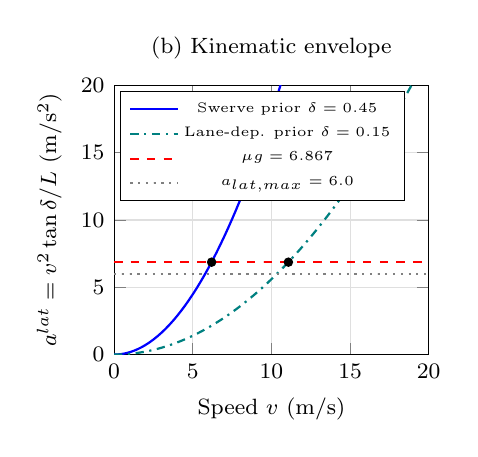
\begin{tikzpicture}
\begin{axis}[
    width=0.46\linewidth, height=5.0cm,
    xlabel={Speed $v$ (m/s)}, ylabel={$a^{\text{lat}} = v^2 \tan\delta / L$ (m/s$^2$)},
    xmin=0, xmax=20, ymin=0, ymax=20, domain=0:20, samples=81,
    restrict y to domain=0:25,
    legend style={font=\tiny, at={(0.02,0.98)}, anchor=north west},
    tick label style={font=\footnotesize}, label style={font=\footnotesize},
    grid=major, grid style={gray!25},
    title={\footnotesize (b) Kinematic envelope}]
\addplot[thick, blue] {x^2*0.48306/2.7};
\addlegendentry{Swerve prior $\delta = 0.45$}
\addplot[thick, teal, dashdotted] {x^2*0.15114/2.7};
\addlegendentry{Lane-dep. prior $\delta = 0.15$}
\addplot[thick, red, dashed, domain=0:20] {6.867};
\addlegendentry{$\mu g = 6.867$}
\addplot[thick, gray, dotted, domain=0:20] {6.0};
\addlegendentry{$a_{\text{lat,max}} = 6.0$}
\addplot[only marks, mark=*, mark size=1.5pt] coordinates {(6.20,6.867) (11.08,6.867)};
\end{axis}
\end{tikzpicture}
\captionsetup{singlelinecheck = false, format= hang, justification=justified, font=footnotesize, labelsep=space}
\caption{PIKV validation analysis: (a) pruning rate per mode; (b) lateral acceleration envelope ($L=2.7$~m).}
\label{fig_pikv}
\end{figure}

The rejection pattern depends on the kinematic limits configured for this experiment. The straight-braking prior of $-5$~m/s$^2$ stays below the configured friction limit of $6.867$~m/s$^2$, so none of those hypotheses were removed. With the sharp-swerve setting ($\delta = 0.45$), the lateral-acceleration curve crosses the same limit at about 22~km/h (6.2~m/s); this is consistent with the high rejection rate at the tested speeds. Left and right swerves still differ: PIKV rejected 70.8\% of left-swerve hypotheses and 21.2\% of right-swerve hypotheses, although their priors were symmetric. Decoder residuals or dataset bias may explain the difference. All sudden-acceleration hypotheses were rejected because the learned steering residuals pushed total acceleration above $\mu g$.

\subsection{Ablation Study and Risk Analysis}
We compared five model configurations on the 120-sample validation subset. Table~\ref{table_ablation} reports their accuracy, FPR, and per-sample latency.

\begin{table}[H]
\caption{Ablation study on the 120-sample validation split (anomaly threshold CRT $> 0.4$).}
\centering
\label{table_ablation}
\adjustbox{max width=\linewidth}{
\begin{tabular}{l|c|c|c}
\hline
\textbf{Configuration} & \textbf{Accuracy (\%)} & \textbf{FPR (\%)} & \textbf{Latency / sample (ms)} \\
\hline
Reactive TTC-Only Baseline (anomaly if $\min_i \text{TTC}_i < 3$~s) & 94.2 & 100.0 & 0.08 \\
Scene Graph Attention only (No CF, No PIKV) & 5.8 & 0.0 & 0.20 \\
CSGA without PIKV (unconstrained counterfactuals) & 100.0 & 0.0 & 0.51 \\
CSGA + PIKV without causal gate input & 100.0 & 0.0 & 0.51 \\
\textbf{PC-CSG Full (CSGA + PIKV + causal gate head)} & \textbf{100.0} & \textbf{0.0} & \textbf{0.92} \\
\hline
\end{tabular}
}
\end{table}

The ablation timings do not align directly with the component-level profile in Table~\ref{table_latency}: for example, the ablation table reports 0.51~ms for CSGA without PIKV, while the component profile reports 1.57~ms for CSGA and 0.53~ms for PIKV. The supplied experiment notes do not specify whether the timers cover the same operations or use the same measurement procedure, so the figures should not be treated as a like-for-like timing decomposition until those conditions are clarified.

% TODO before submission: document the timing protocol for both tables (including warm-up, batch size, synchronisation, and which operations are included) and reconcile these figures if they are intended to be directly comparable.

The 120-scene subset is strongly imbalanced. The reactive TTC baseline labelled every sample as an anomaly, producing 94.2\% accuracy and 100\% FPR. Scene-graph attention alone predicted no anomalies; its accuracy was 5.8\% and its FPR was 0\%. In this subset, about 94.2\% of the samples are hazard scenes and only 5.8\% (seven scenes) are benign. The accuracy of the TTC baseline therefore comes from predicting the majority class, not from separating safe cases from hazardous ones. The counterfactual variants classified all 120 samples correctly, but a larger and more balanced test set is needed to determine whether this result generalises.

Because only seven scenes are benign, this subset cannot establish an empirical reduction in FPR due to PIKV. Proposition~2 states that PIKV cannot increase FPR, but the current experiment does not show a measured reduction. The causal gate also made no difference in this ablation: its scores are computed, but they are not yet multiplied into the attention weights.

Figure~\ref{fig_scenarios} shows the four scripted cases. In Scenarios B--D, CRT follows the hazard curve $H(\text{TTC})$. Under the current gate, $H \ge 0.25$ requires $\text{TTC} \le 3.55$~s. A Level~1 alert therefore cannot be raised when TTC is above 3.55~s; this limit follows from the present threshold setting.

\begin{table}[H]
\caption{Measured behaviour of PC-CSG on the four scripted demo scenarios.}
\centering
\label{table_scenarios}
\adjustbox{max width=\linewidth}{
\begin{tabular}{l|l|c|c|c|l}
\hline
\textbf{Scenario} & \textbf{Driving Context} & \textbf{Ego Speed} & \textbf{Worst TTC} & \textbf{CRT} & \textbf{Level / Action} \\
\hline
A & Highway cruise, all clear & 100.1~km/h & 33.3~s & 0.000 & Level 0: nominal cruise \\
B & Lead vehicle decelerating & 110.2~km/h & 4.1~s & 0.103 & Level 0: monitoring \\
C & Lane-change swerve conflict & 119.9~km/h & 1.9~s & 0.894 & Level 4: AEB + MRM \\
D & Barrier + hard lead braking & 100.1~km/h & 0.5~s & 0.987 & Level 4: full AEB \\
\hline
\end{tabular}
}
\end{table}

\begin{figure}[H]
\centering
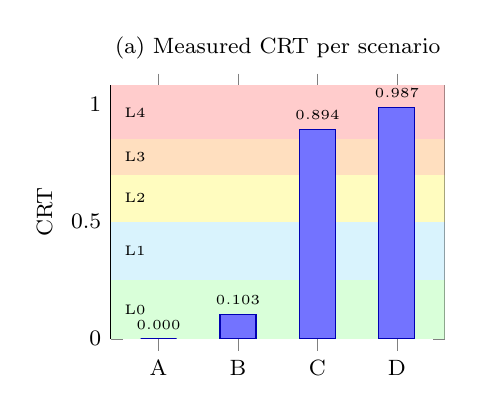
\begin{tikzpicture}
\begin{axis}[
    ybar, width=0.48\linewidth, height=4.8cm,
    ylabel={CRT}, ymin=0, ymax=1.08,
    xtick={1,2,3,4}, xticklabels={A, B, C, D},
    xmin=0.4, xmax=4.6, bar width=13pt,
    nodes near coords={\pgfmathprintnumber[fixed, fixed zerofill, precision=3]{\pgfplotspointmeta}},
    every node near coord/.append style={font=\tiny},
    tick label style={font=\footnotesize}, label style={font=\footnotesize},
    title={\footnotesize (a) Measured CRT per scenario}]
\fill[green!15] (axis cs:0.4,0) rectangle (axis cs:4.6,0.25);
\fill[cyan!15] (axis cs:0.4,0.25) rectangle (axis cs:4.6,0.50);
\fill[yellow!25] (axis cs:0.4,0.50) rectangle (axis cs:4.6,0.70);
\fill[orange!25] (axis cs:0.4,0.70) rectangle (axis cs:4.6,0.85);
\fill[red!20] (axis cs:0.4,0.85) rectangle (axis cs:4.6,1.08);
\node[font=\tiny, anchor=west] at (axis cs:0.45,0.125) {L0};
\node[font=\tiny, anchor=west] at (axis cs:0.45,0.375) {L1};
\node[font=\tiny, anchor=west] at (axis cs:0.45,0.60) {L2};
\node[font=\tiny, anchor=west] at (axis cs:0.45,0.775) {L3};
\node[font=\tiny, anchor=west] at (axis cs:0.45,0.965) {L4};
\addplot[fill=blue!55, draw=blue!70!black] coordinates {(1,0.000) (2,0.103) (3,0.894) (4,0.987)};
\end{axis}
\end{tikzpicture}
\hfill
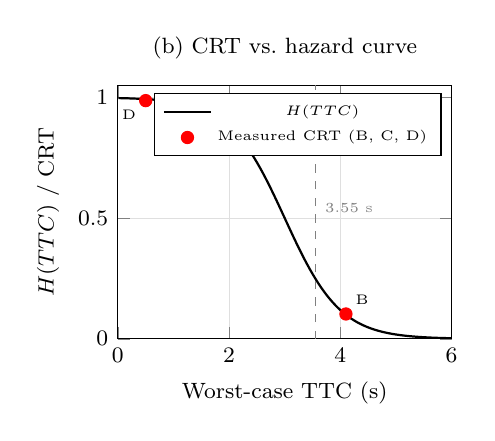
\begin{tikzpicture}
\begin{axis}[
    width=0.48\linewidth, height=4.8cm,
    xlabel={Worst-case TTC (s)}, ylabel={$H(\text{TTC})$ / CRT},
    xmin=0, xmax=6, ymin=0, ymax=1.05, domain=0.01:6, samples=121,
    legend style={font=\tiny}, legend pos=north east,
    tick label style={font=\footnotesize}, label style={font=\footnotesize},
    grid=major, grid style={gray!25},
    title={\footnotesize (b) CRT vs.\ hazard curve}]
\addplot[thick, black] {1/(1+exp((x-3.0)/0.5))};
\addlegendentry{$H(\text{TTC})$}
\addplot[only marks, mark=*, mark size=2.2pt, red] coordinates {(4.1,0.103) (1.9,0.894) (0.5,0.987)};
\addlegendentry{Measured CRT (B, C, D)}
\addplot[thin, gray, dashed] coordinates {(3.55,0) (3.55,1.05)};
\node[font=\tiny, anchor=south west] at (axis cs:4.1,0.103) {B};
\node[font=\tiny, anchor=south west] at (axis cs:1.9,0.894) {C};
\node[font=\tiny, anchor=north east] at (axis cs:0.5,0.987) {D};
\node[font=\tiny, anchor=north west, gray] at (axis cs:3.55,0.6) {3.55 s};
\end{axis}
\end{tikzpicture}
\captionsetup{singlelinecheck = false, format= hang, justification=justified, font=footnotesize, labelsep=space}
\caption{Demo scenarios: (a) CRT values and intervention bands; (b) CRT vs.\ hazard curve.}
\label{fig_scenarios}
\end{figure}

\subsection{Capability Comparison with Related Methods}
The methods reviewed here address different tasks, from trajectory prediction to offline testing. We did not evaluate them on a shared dataset, so an accuracy comparison would not be reliable. Table~\ref{table_comparison} instead summarises the capabilities described in the cited papers.

\begin{table}[H]
\caption{Capability comparison with related methods, based on the descriptions in the original papers. Latency is given only for PC-CSG because the other papers do not report it on comparable hardware.}
\centering
\label{table_comparison}
\adjustbox{max width=\linewidth}{
\begin{tabular}{l|c|c|c|c|c|l}
\hline
\textbf{Method} & \textbf{Venue / Year} & \textbf{Counterfactual Hypotheses} & \textbf{Physics Check} & \textbf{Interaction Structure} & \textbf{Risk $\rightarrow$ Action} & \textbf{Setting} \\
\hline
TTC-only baseline & -- & No & No & No & Binary & Online, reactive \\
CRiTIC \cite{ahmadi2025critic} & ICRA 2025 & No & No & Causal gating & No & Online prediction \\
CICR \cite{han2025cicr} & J. Imaging 2025 & Yes (counterfactual decoder) & No & Social context & No & Pedestrian prediction \\
Liao et al. \cite{liao2024physics} & IJCAI 2024 & No & Bicycle model & Interaction encoder & No & Prediction \\
TPK \cite{baden2025tpk} & IV 2025 & No & Kinematic layer & Interaction priors & No & Prediction \\
CounterScene \cite{jing2026counterscene} & arXiv 2026 & Yes (causal agent) & No & Causal interaction graph & No & Offline testing \\
STRAP \cite{ning2025strap} & ITSC 2025 & No & No & Risk-field attention & No & Prediction \\
\hline
\textbf{PC-CSG (ours)} & -- & \textbf{Yes (6 modes)} & \textbf{PIKV (6 checks)} & \textbf{Scene graph} & \textbf{5 levels} & \textbf{Online, 6.68~ms} \\
\hline
\end{tabular}
}
\end{table}

The methods in Table~\ref{table_comparison} cover different parts of the problem. CRiTIC \cite{ahmadi2025critic} selects relevant agents. CICR \cite{han2025cicr} addresses pedestrian trajectory prediction and uses a counterfactual decoder; its front-door criterion is part of the causal-intervention fusion module. CounterScene \cite{jing2026counterscene} also evaluates counterfactual futures, while Liao et al. \cite{liao2024physics} and TPK \cite{baden2025tpk} incorporate constraints related to vehicle motion. Among these selected methods, we did not identify one that combines physics-checked counterfactual risk with graded driver-assistance actions in the perception loop. PC-CSG combines these steps and processed a frame in 6.68~ms on the tested laptop GPU. This is a capability comparison only; forecasting accuracy was not measured on common data. The TTC-only baseline is our reactive reference implementation, with the 3~s cutoff used as an experimental setting rather than a claim about a published method.

\section{Conclusion and future scope} \label{section5}
On the RTX 3050 Laptop GPU, PC-CSG processed a frame in 6.68~ms (149.7~FPS), and PIKV rejected 312 of 678 counterfactual hypotheses (46.0\%). On the 120-sample ablation subset, PC-CSG recorded 100.0\% accuracy and 0.0\% FPR, compared with 94.2\% accuracy and 100.0\% FPR for the reactive TTC baseline. These measurements indicate that the pipeline can run within the tested laptop's timing budget, but they do not establish performance on embedded automotive hardware or generalisation to a broader data distribution. As described in the analysis, PIKV removes friction-violating hypotheses from the risk score, the physics layers are reference-frame independent, and the risk score increases as TTC decreases. Proposition~2 states that PIKV does not increase FPR.

Several limitations remain in the current implementation. The validation subset is small and imbalanced, the causal gate is computed but not applied to the attention weights, and the physics loss currently provides no gradient. The present TTC gate also prevents a Level~1 warning when TTC exceeds about 3.55~s; a reliable warning lead time has not yet been measured. These findings point to two next steps:
\begin{enumerate}
    \item \textbf{Multi-modal counterfactual fusion:} The current evaluation does not test what happens when camera-based information is degraded or unavailable. Extending CSGA to use camera, LiDAR, and radar tracks together, then testing on nuScenes \cite{caesar2020nuscenes} and Waymo Open \cite{sun2020waymo}, would help measure whether the counterfactual scores remain useful in rain, glare, or low light.
    \item \textbf{V2X cooperative counterfactual graphs:} The current scene graph is limited to agents available to the vehicle's own sensors. Sharing scene graphs and CRT values with nearby vehicles or roadside units over Vehicle-to-Everything (V2X) links could add information about agents hidden from those sensors, for example a vehicle behind a truck.
\end{enumerate}

\bibliography{mybibfile}

\end{document}
